\documentclass[a4paper,12pt]{scrartcl}
\usepackage[margin=2.5cm
  %,showframe% <- only to show the page layout
  ]{geometry} % change margin to more compact
%%%%%% header matter %%%%%%
\usepackage[T1]{fontenc}
\usepackage{amsmath}
\usepackage{graphicx}
\usepackage{float}
\usepackage{xcolor}
\usepackage{authblk} % Allows for authors from multiiple institutes
\usepackage{siunitx} % Allow for scientific unit
\usepackage{hyperref}
\hypersetup{colorlinks,%
            citecolor=black,%
            filecolor=black,%
            linkcolor=black,% link like content or so
            urlcolor=blue,%
            pdftex}
\usepackage{lineno} % to use \linenumbers
\linenumbers % give line number as a draft version
%%%%%% start: code style %%%%%%

\usepackage{listings}
%\usepackage{color}
\definecolor{codegreen}{rgb}{0,0.6,0}
\definecolor{codegray}{rgb}{0.5,0.5,0.5}
\definecolor{codepurple}{rgb}{0.58,0,0.82}
\definecolor{backcolour}{rgb}{0.95,0.95,0.92}

\lstdefinestyle{mystyle}{
    backgroundcolor=\color{backcolour},
    commentstyle=\color{codegreen},
    keywordstyle=\color{magenta},
    numberstyle=\tiny\color{codegray},
    stringstyle=\color{codepurple},
    basicstyle=\footnotesize,
    breakatwhitespace=false,
    breaklines=true,
    captionpos=b,
    keepspaces=true,
    numbers=left,
    numbersep=5pt,
    showspaces=false,
    showstringspaces=false,
    showtabs=false,
    tabsize=2
}

\lstset{style=mystyle}
%%%%%% end: code style %%%%%%

%%%%%% header matter %%%%%%

\title{
\includegraphics[width=10cm]{DESYTestBeam.png}  
\includegraphics[width=10cm]{Aida2020.png} \\ \vspace{2cm} USER MANUAL \\ Slow Control System}
\author[*]{Lars Fischer}
\author[*]{Mengqing Wu}
\affil[*]{Deutsches Elektronen-Synchrotron DESY, Notkestr. 85, 22607 Hamburg, Germany}

\date{\today}

\begin{document}
\clearpage\maketitle
This document serves as a how-to manual for the common environmental Slow Control System at DESY test beam facility. This system is has a rack-based hardware, connecting to the test beam common DAQ, EUDAQ2, via a SQL DataBase, MySQL.
Its hardware and software will be introduced briefly, with a focus on the following concepts:
a step-by-step instruction of the installation and the configuration of the software;
a easy-to-follow guide for users who wish to integrate their own slow control inputs to our system, or to the common EUDAQ2 datastream.
\thispagestyle{empty}
\cleardoublepage

\tableofcontents
\pagebreak

\section{Introduction}
\subsection{Hardware and software}
The Slow Control System is currently able to collect connected sensor data in a configurable frequence (i.e. how frequent to update the DataBase variables from sensor data), transfer to the test beam common DAQ, EUDAQ2, and finally write to user data taking events as a standard EUDAQ raw event tag, i.e. not affecting any user customized event definition.
For further reading, a detailed description of the system design and a manual for developers, please see the following documents:
\begin{itemize}
  \item Deliverable Report: \href{https://cds.cern.ch/record/2290758/files/AIDA-2020-D15\_3.3.pdf}{\footnotesize{https://cds.cern.ch/record/2290758/files/AIDA-2020-D15\_3.3.pdf}};
  \item Main User Manual: \href{https://cds.cern.ch/record/2284369/files/AIDA-2020-NOTE-2017-007.pdf}{\footnotesize{https://cds.cern.ch/record/2284369/files/AIDA-2020-NOTE-2017-007.pdf}}.
\end{itemize}
This document will guide you step by step through the software design and all necessary installations.


\subsubsection*{Rack and sensors}
The DAQ system hardware is a rack-based system which is movable and connected via an Ethernet cable, as shown in Figure~\ref{fig:sc-rack}; it is currently equipped with \textbf{10 NTC sensors} for temperature measurements in an operation range of \SI{-20}{\celsius} to \SI{+100}{celsius} \footnote{NB: to be confirmed, not sure where Lars found this info...}, and \textbf{one DIGI sensor} for complimentary measurements of air pressure, dew point and humidity.
\begin{figure}[!ht]
  \centering
  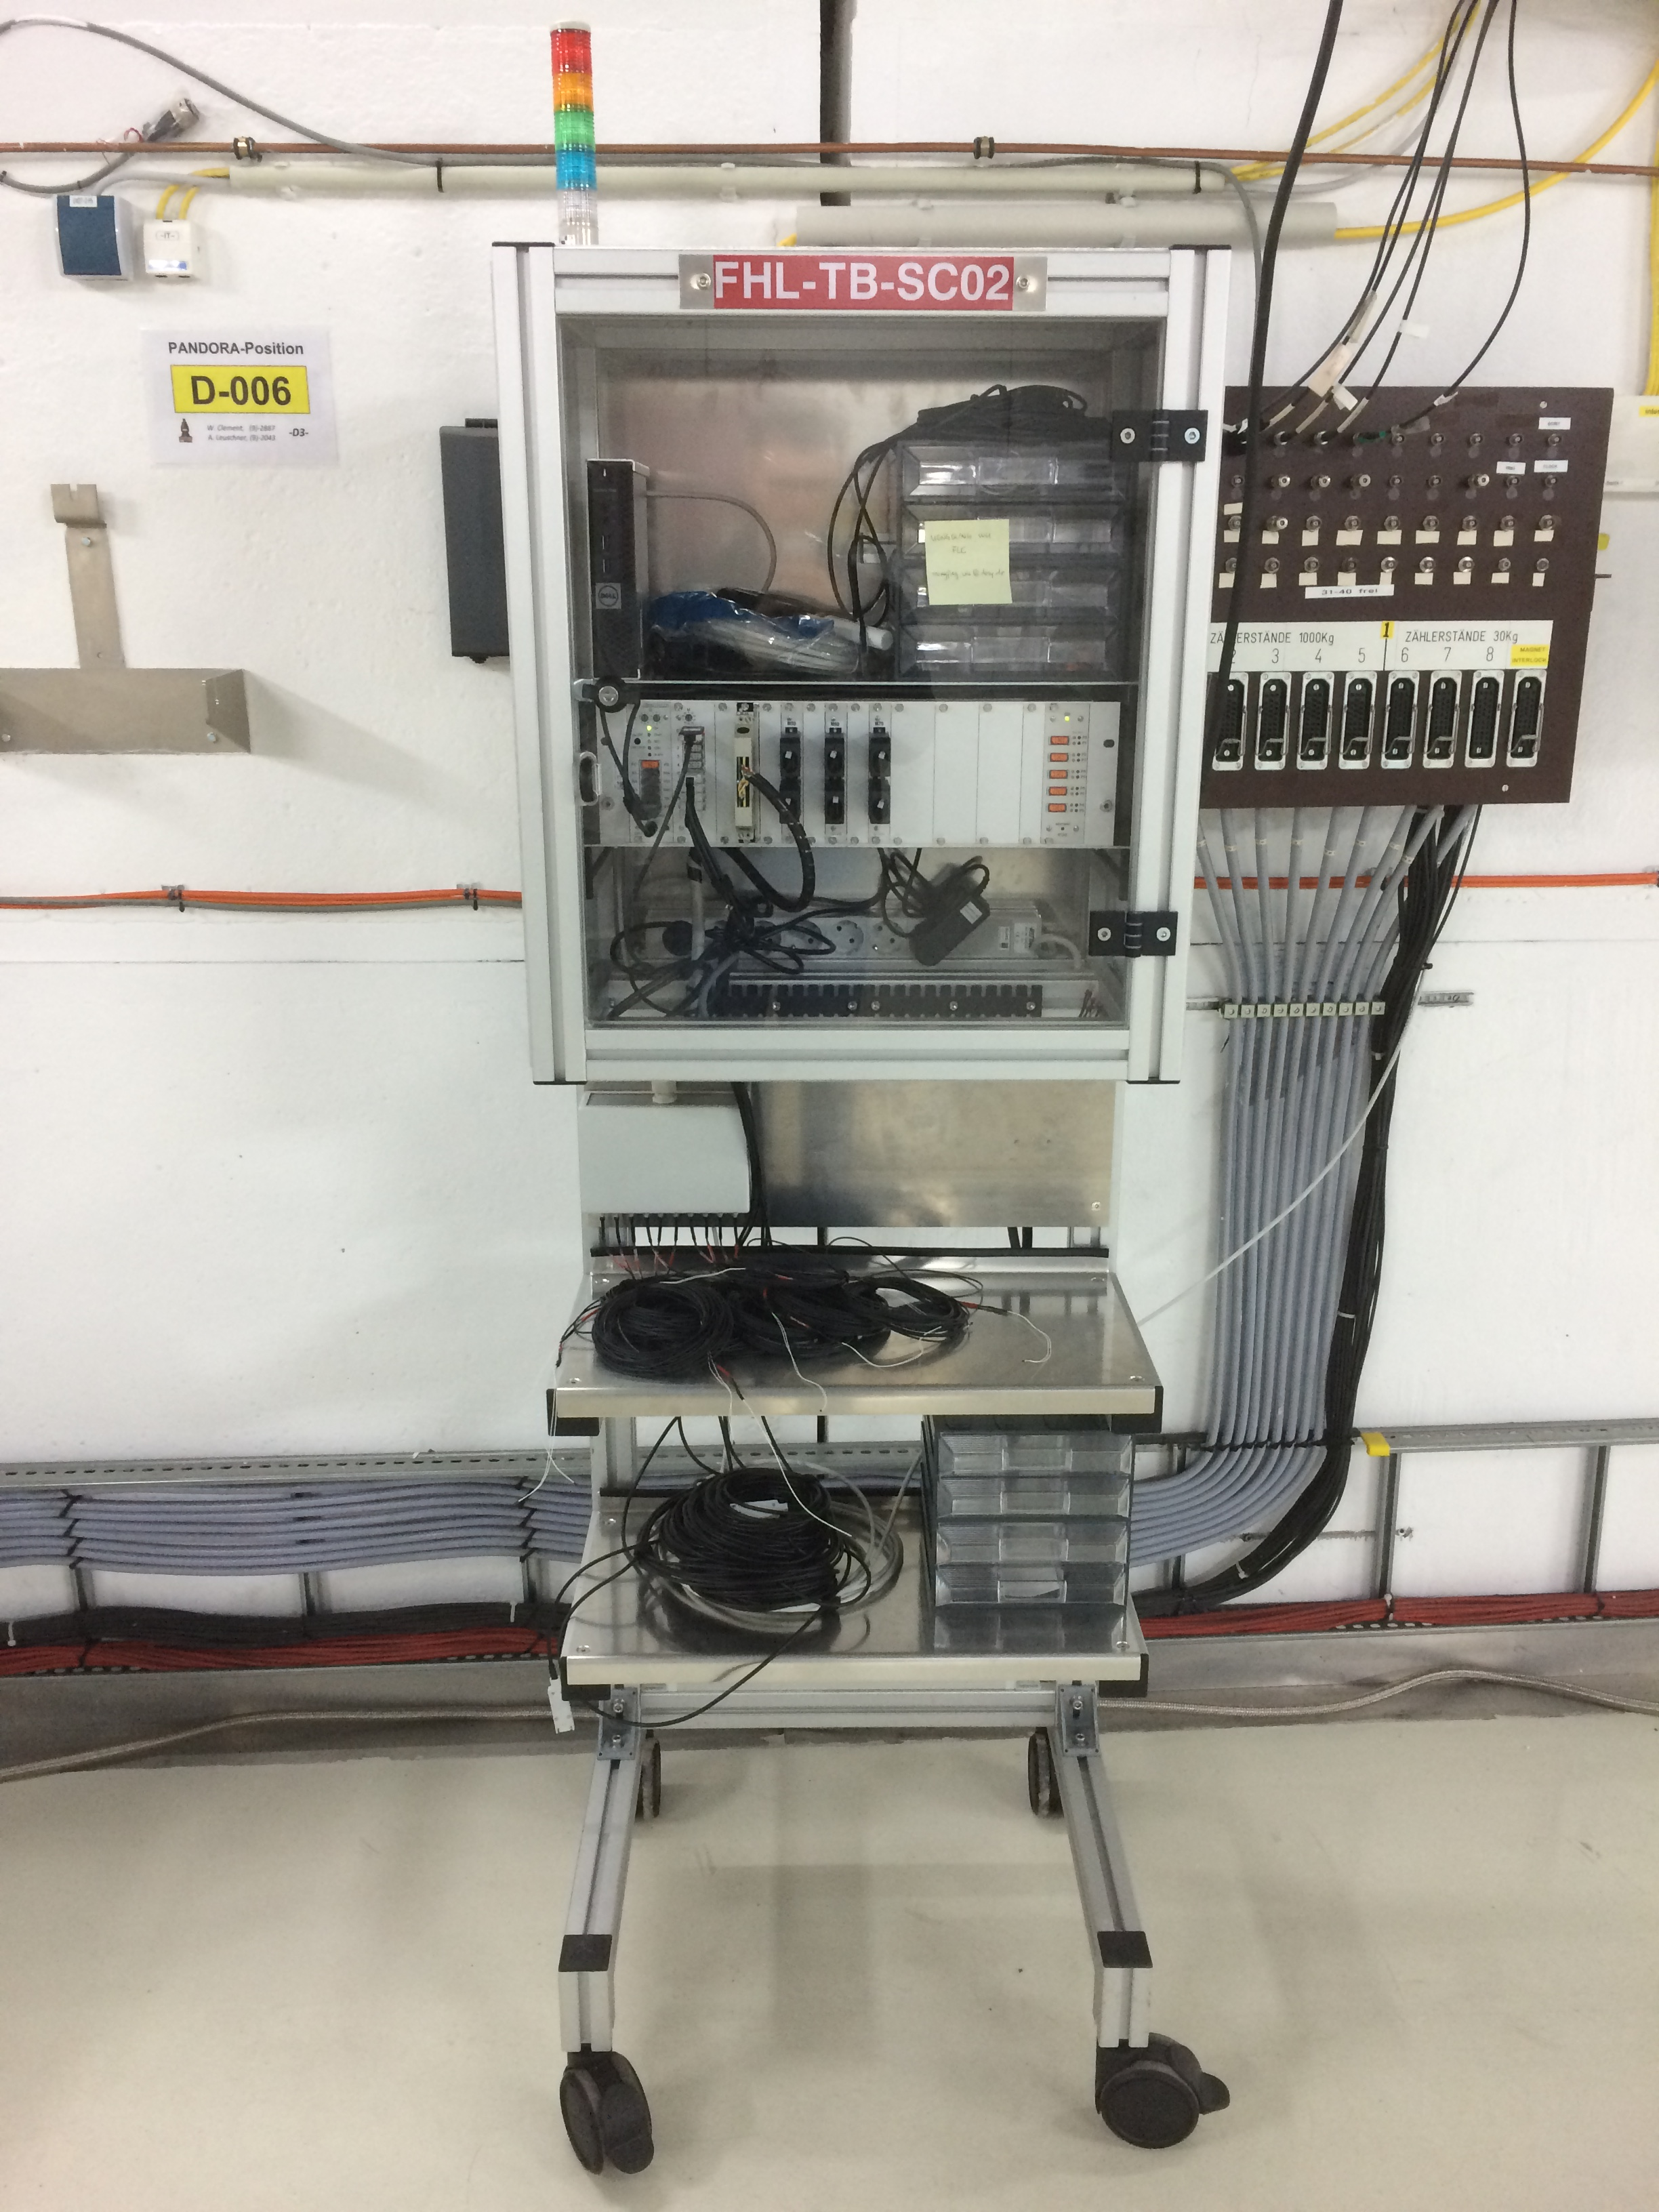
\includegraphics[height=7cm]{Rackganz.jpg}%
  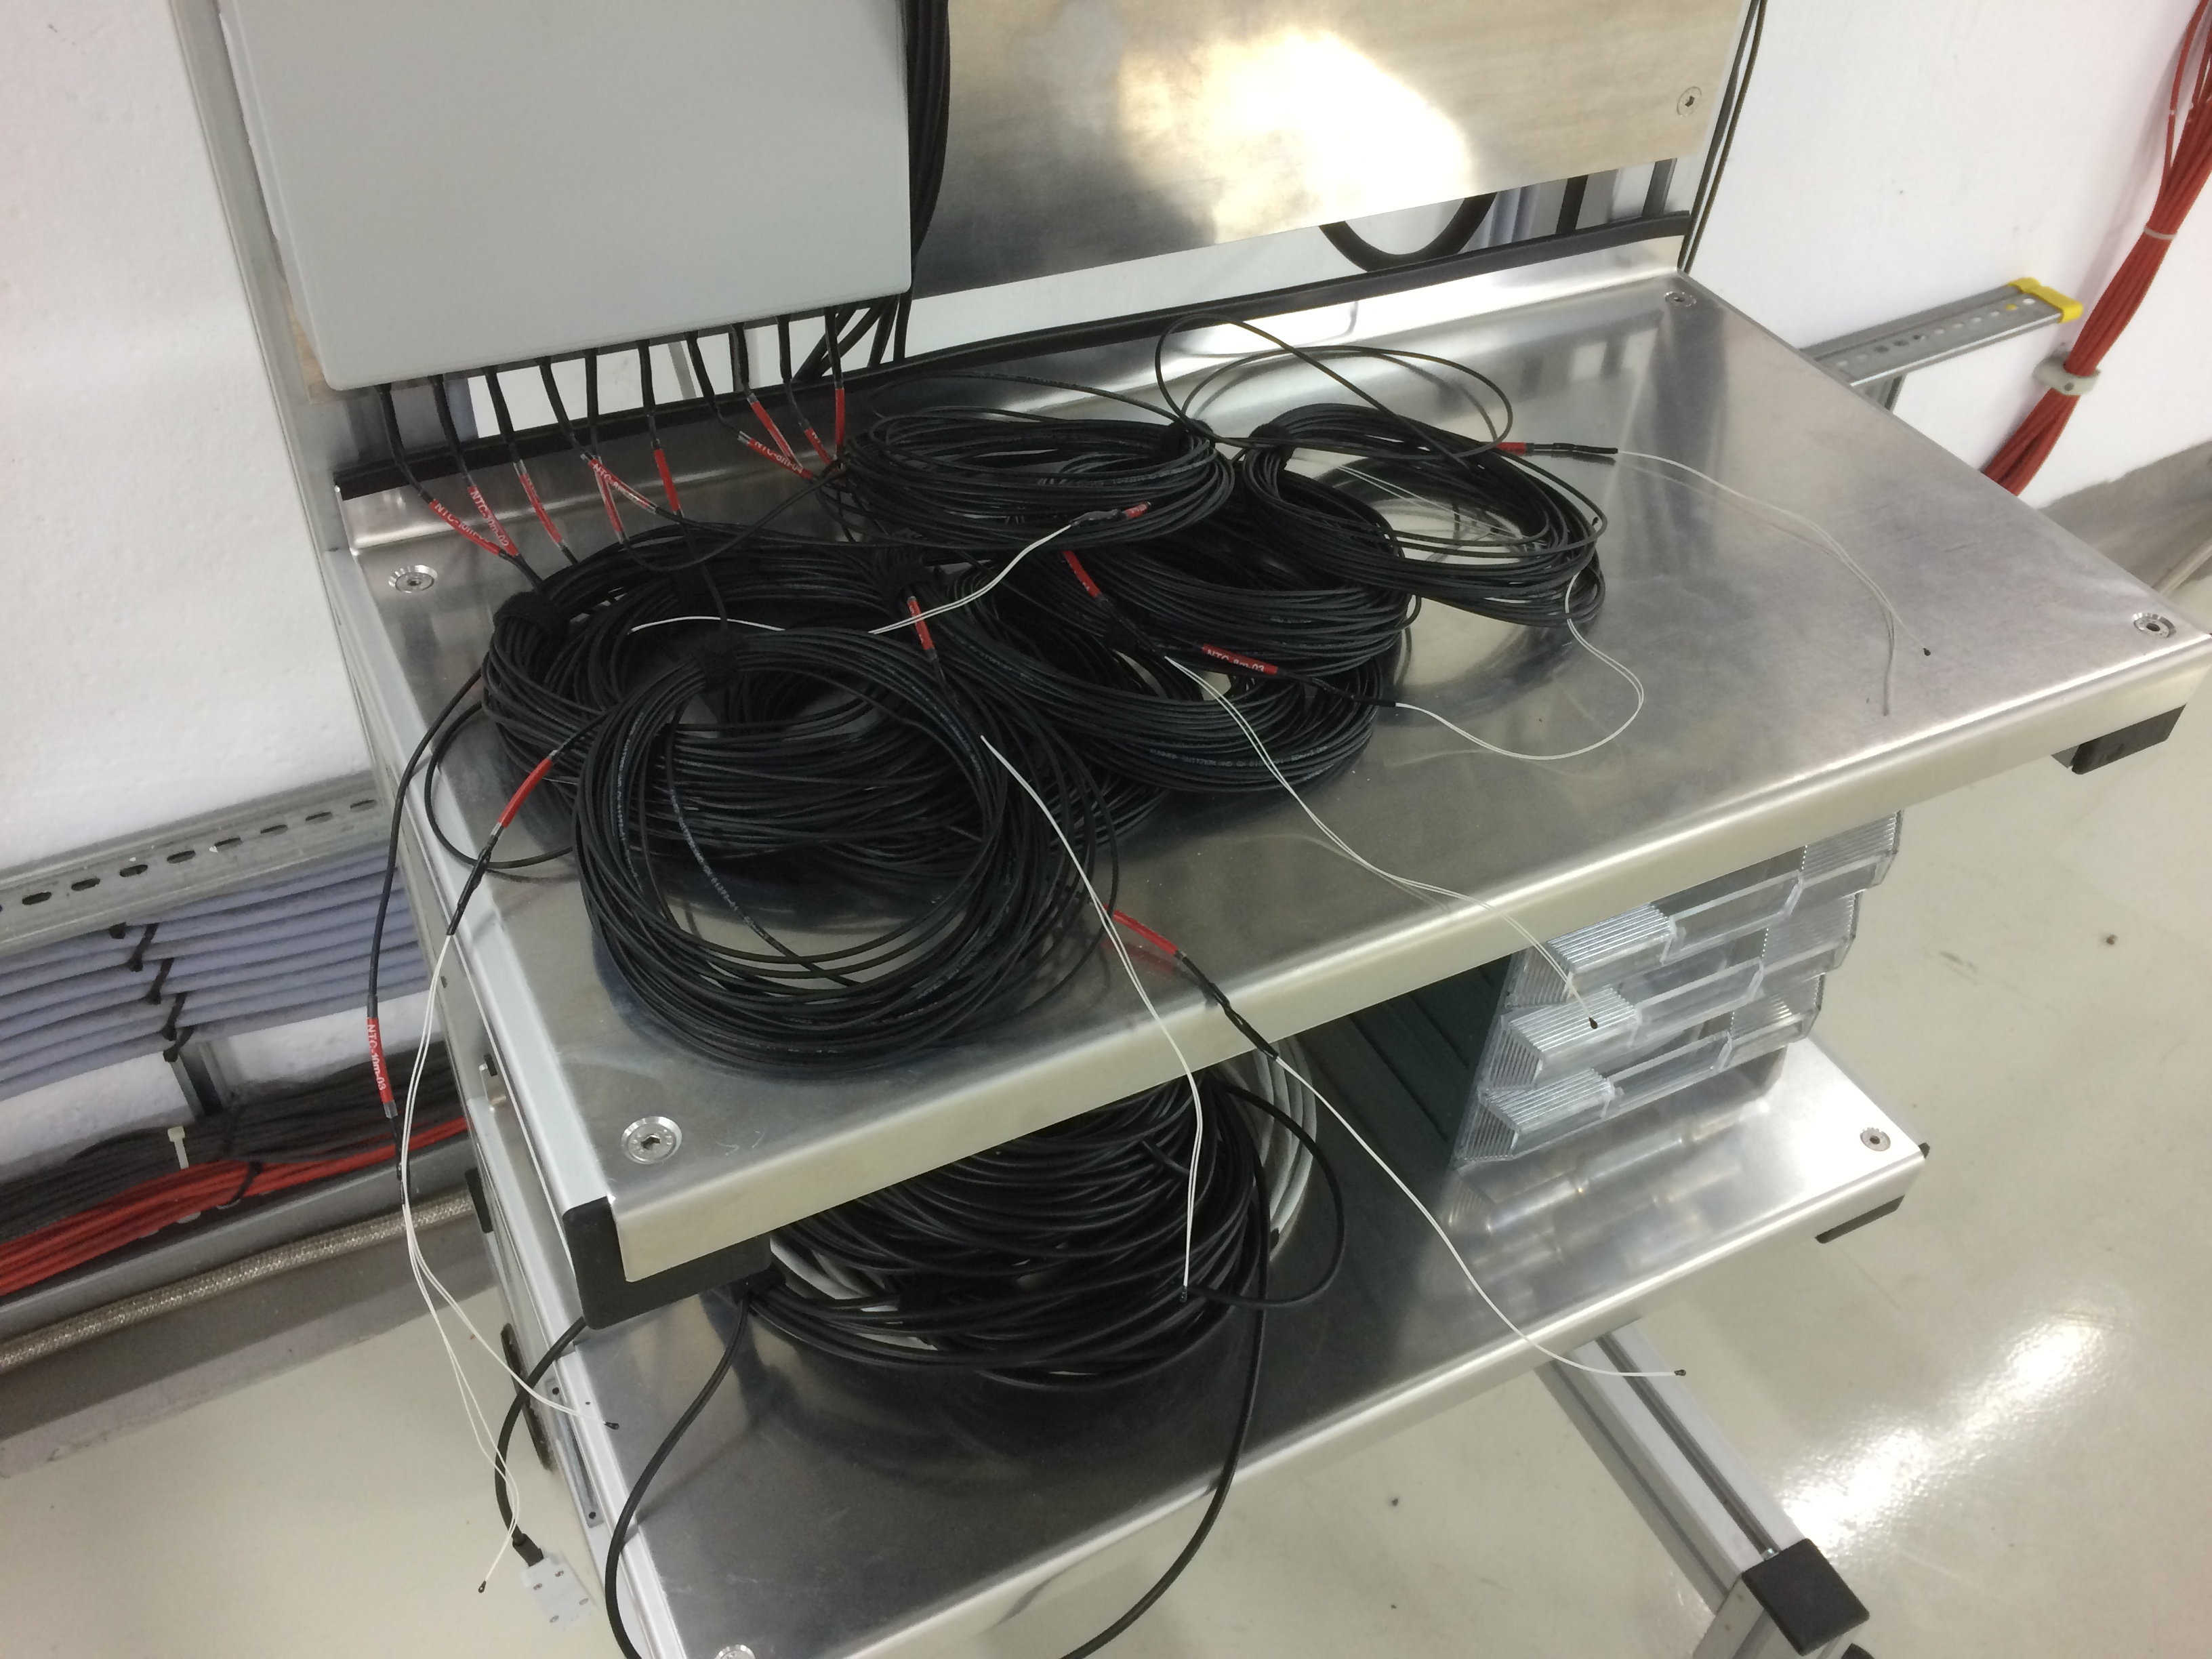
\includegraphics[height=7cm]{Sensoren.jpg}
\caption{Slow Control System rack \#02 (left) in DESY test beam area TB24 and the 10 NTC sensors of \SI{10}{m} long (right).}
\label{fig:sc-rack}
\end{figure}

The NTC sensors are \SI{10}{m} long that can be located at different measuring points in a beam area, according to user needs; the DIGI sensor is fixed at the rear of the rack, and can be used as alarm monitor~\footnote{There is \textbf{a LED-based alarm} available on the rack (seated on the top of the rack), however, it is not yet plugged to test; users are also able to use it with their defined warning signals.}. All the sensors are connected to a data logger (ALMEMO) via a special connector. Users are also able to \textbf{mount their own sensors} to the data collector, with many spared connectors stored on the rack, but \textbf{please contact the local support team before any customized modification to the system!}

\subsubsection*{Software}
The DAQ software consists of \textbf{a commercial DAQ (AMR)} and a testbeam common DAQ software, \textbf{EUDAQ2}.
The data logger is connected to a Windows-PC mounted on the rack, and it is polled via a USB connector by a commercial DAQ software (AMR) provided by the same company.

This document will give a detailed instruction to guide you to configure and to use the DAQ system to get a measurement based on the connected sensors.

\subsection{Status and Note for usage}
The DESY test beam facility includes three beam areas, TB21, TB22, with TB24 and TB24/1 in tandem as shown in Figure~\ref{fig:desytb}. \textbf{Two} Slow Control racks are currently available to move around at the test beam for different use cases.

\begin{figure}[!ht]
  \centering
  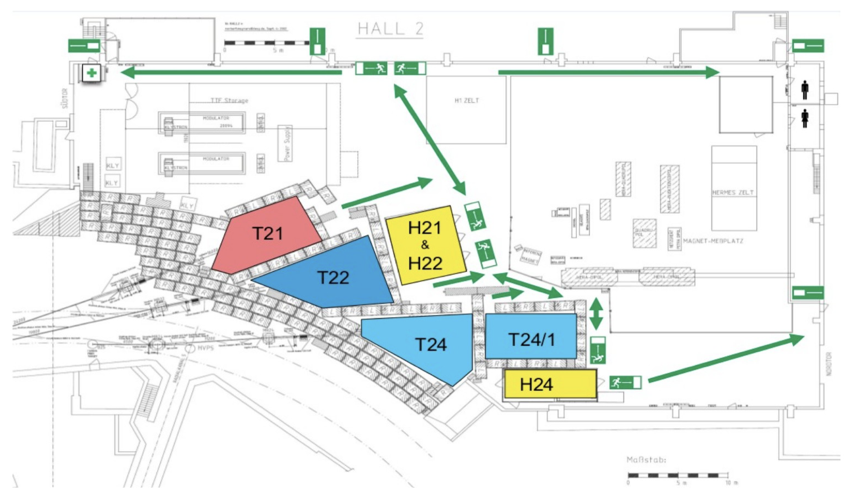
\includegraphics[width=0.8\textwidth]{Testbeam.png}
\caption{Slow Control System Racks can be moved in T21/T22/T24 for observing.}
\label{fig:desytb}
\end{figure}

The power and Internet connection should always be connected, while the Slow Control System is in use. Once the power was off, in order to continue the slow control data streaming, one needs to: 1) release the beam area interlock; 2) check to ensure the data logger is on, and the PC is on.

You can of course do the following things, however, please kindly inform the contact person \textbf{before}:
\begin{itemize}
  \item disconnect the Ethernet cable and/or unpower the slow control system;
  \item replace the NTC sensors;
  \item relocate the rack by rolling it among different test beam areas or even to other work space;
\end{itemize}

\section{The Ready-to-use DAQ}
\subsection{Structure}
The system data acquisition (DAQ) is implemented by two PCs running in parallel, see Figure~\ref{fig:DAQflow}.
The DAQ is developped based on the current hardware, that user only needs to: 1) load a testbeam slow control \textit{Producer} module in EUDAQ2 as you will do to load your device; 2) copy/paste the prepared slow control config file to your config file; 3) run the EUDAQ2 like how you will do to take data from your device. At the end of the run, once all the data is written to a standard EUDAQ2 raw file, you can find all the slow control data recorded as tags in your event.

\begin{figure}[!ht] \centering
%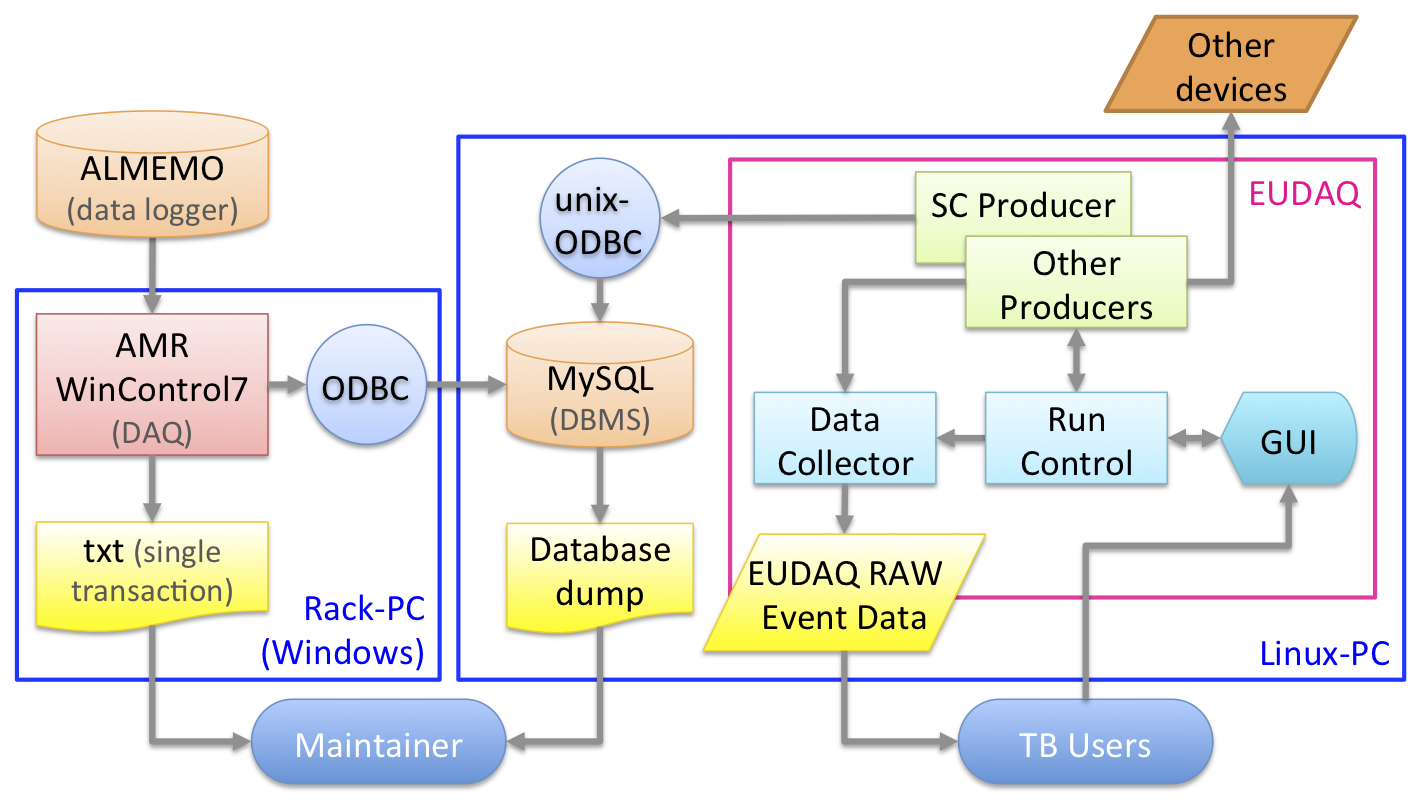
\includegraphics[trim={5cm .5cm 2cm 5cm},clip,width=\textwidth]{FlowChartSCS.png}
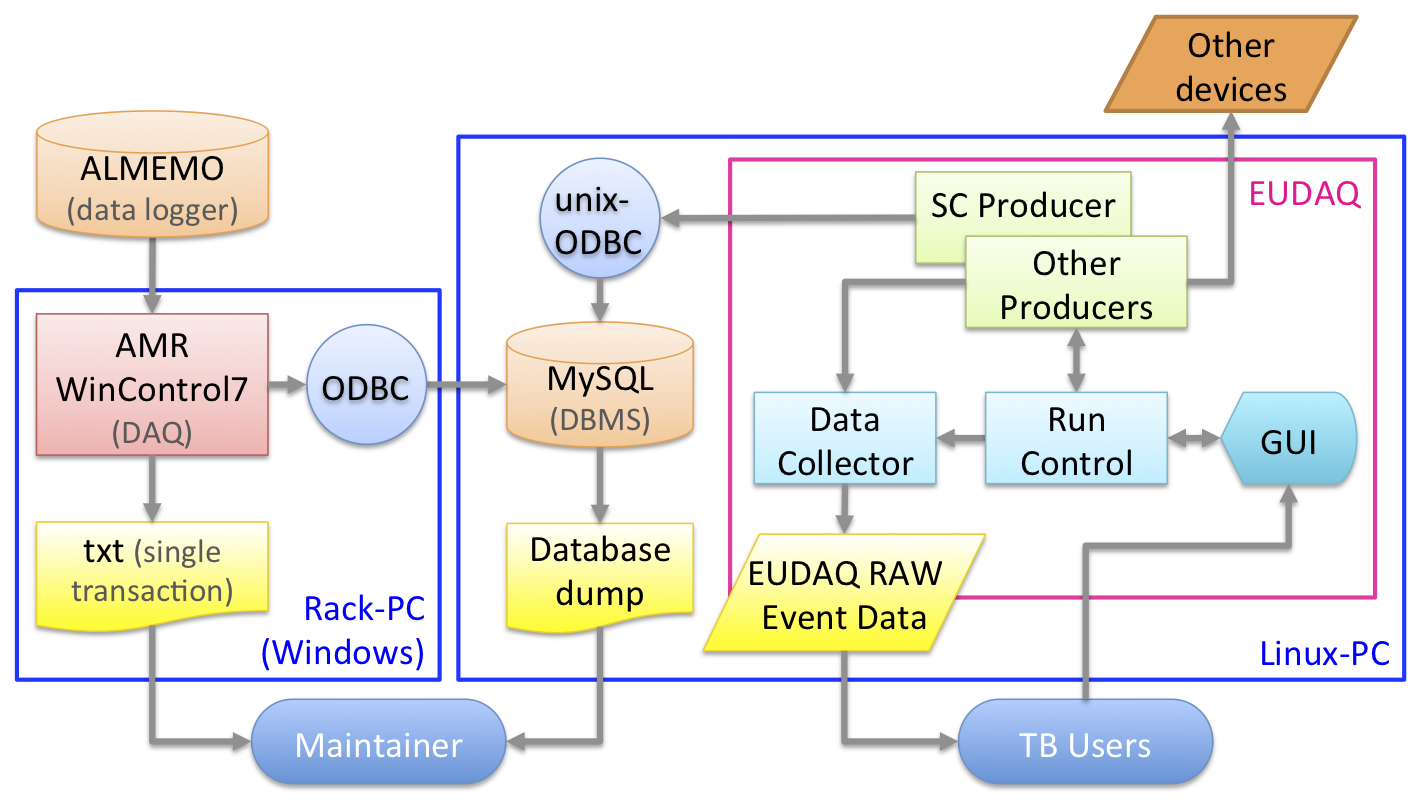
\includegraphics[width=0.85\textwidth]{FlowChartSCS.png}
\caption{Flow chart of the Slow Control System}
\label{fig:DAQflow}
\end{figure}

\subsection{Windows Rack PC}
The Windows PC on the rack collects the data from data logger (ALMEMO) with a commercial DAQ software (AMR).
With a default (updated in Jan 2018) configuration: AMR software polls data from data logger every \SI{30}{s}.
An ODBC is set up to forward the values into a MySQL (version 5.7.20) based database on the Linux-PC.

\subsection{Linux PC}
The ODBC connector shown in Figure~\ref{fig:DAQflow} connects the Windows Operating System (OS) with any remote DataBase (DB) using the DB's TCP/IP address. Therefore, if the internect connection of either of the two PCs is disconnected, no data can be transferred to the User.

A MySQL Database with necessary tables are set on a Linux PC at DESY, in order to transfer all the connected sensor channels; the relevant setup to send data out from the Windows PC is also prepared. As long as the Windows PC starts to Poll and send out data, the relevant tables in the MySQL DataBase will be filled with entries ordered by timestampes, if both PCs are on and connected to the Internet with their IP addresses not changed).

The EUDAQ2 software is installed on this Linux PC, and it reads out entries from the MySQL tables.
A unix-ODBC is installed to connect the MySQL database with the EUDAQ2 framework.
User can use the EUDAQ2 GUI with prepared Producer and Data collector modules loaded via a command line command, and once User start one EUDAQ2 run with all the relevant GUI, the slow control data will be written down to the standard EUDAQ raw event as tags.
%The EUDAQ software collects data in user defined timestamps from the database on the Linux PC.
%While the data is transfered into the database the second DAQ software collects only the events of the timestamps the user adjusted. The EUDAQ can simply be handled by an own GUI.
After data taking the output can be converted from EUDAQ raw/native file into a readable csv file, with a provided command line converter. Furthermore, there are macros provided to plot the csv data.

\section{Software Setup}
There are \textbf{two APIs} and \textbf{three softwares} to install and to configure:
\begin{itemize}
  \item API:
  \begin{itemize}
    \item ODBC: 32-bit needed, installed by default in Windows, need to install MySQL driver and configure a DSN for the remote MySQL DB;
    \item unixODBC: installation needed, as well as a MySQL driver to install and a DSN to add/configure for connection to MySQL DataBase;
  \end{itemize}

  \item Software:
  \begin{itemize}
    \item AMR: installed under purchase on the Windows Rack PC, ODBC DSN entry needed to add/configure for data transmit (Tx);
    \item MySQL: installation needed, needs to add target DataBase with tables to receive (Rx) data sent from AMR;
    \item EUDAQ2: installation needed, modules and configuration prepared for default setup; configurable variables in .conf files, to change DataBase and/or target tables.
  \end{itemize}
\end{itemize}

\subsection{MySQL}
The MySQL database on the Linux PC is the central interaction point of the two DAQ softwares. First of all there has to be a user which can be used from multiple hostes. This is required so that the AMR software on the Windows PC can remotly access the database. Therefore the certain user has to get access privileges from different computers.

\subsubsection*{Installation}

Install the MySQL server by using the Ubuntu package manage:
\begin{lstlisting}[language=bash]
sudo apt-get updated
sudo apt-get install mysql-server
\end{lstlisting}

After the installtion, run the \verb|mysql_secure_installation| utility, with which you can define the MySQL root user password, configure remote access and etc.
It is simple to start the MySQL shell as the root user with the password you just set:
%\colorbox{lightgray}{\texttt{mysql -u username -p}} \\
\begin{lstlisting}[language=SQL]
mysql -u root -p
mysql>
\end{lstlisting}

\subsubsection*{Remote access configuration}
There are at least two users needed in MySQL, one is write-only for the AMR to access the DataBase and the other is read-only for the EUDAQ2.
You can check all the users with the corresponding hosts using the following command:
%\colorbox{lightgray}{\texttt{mysql> SELECT user, host FROM mysql.user;}}\\
\begin{lstlisting}[language=SQL]
mysql> SELECT user, host FROM mysql.user;
\end{lstlisting}

Then you should see an output as shown in Figure~\ref{fig:mysql-user}:
\begin{figure}[!ht] \centering
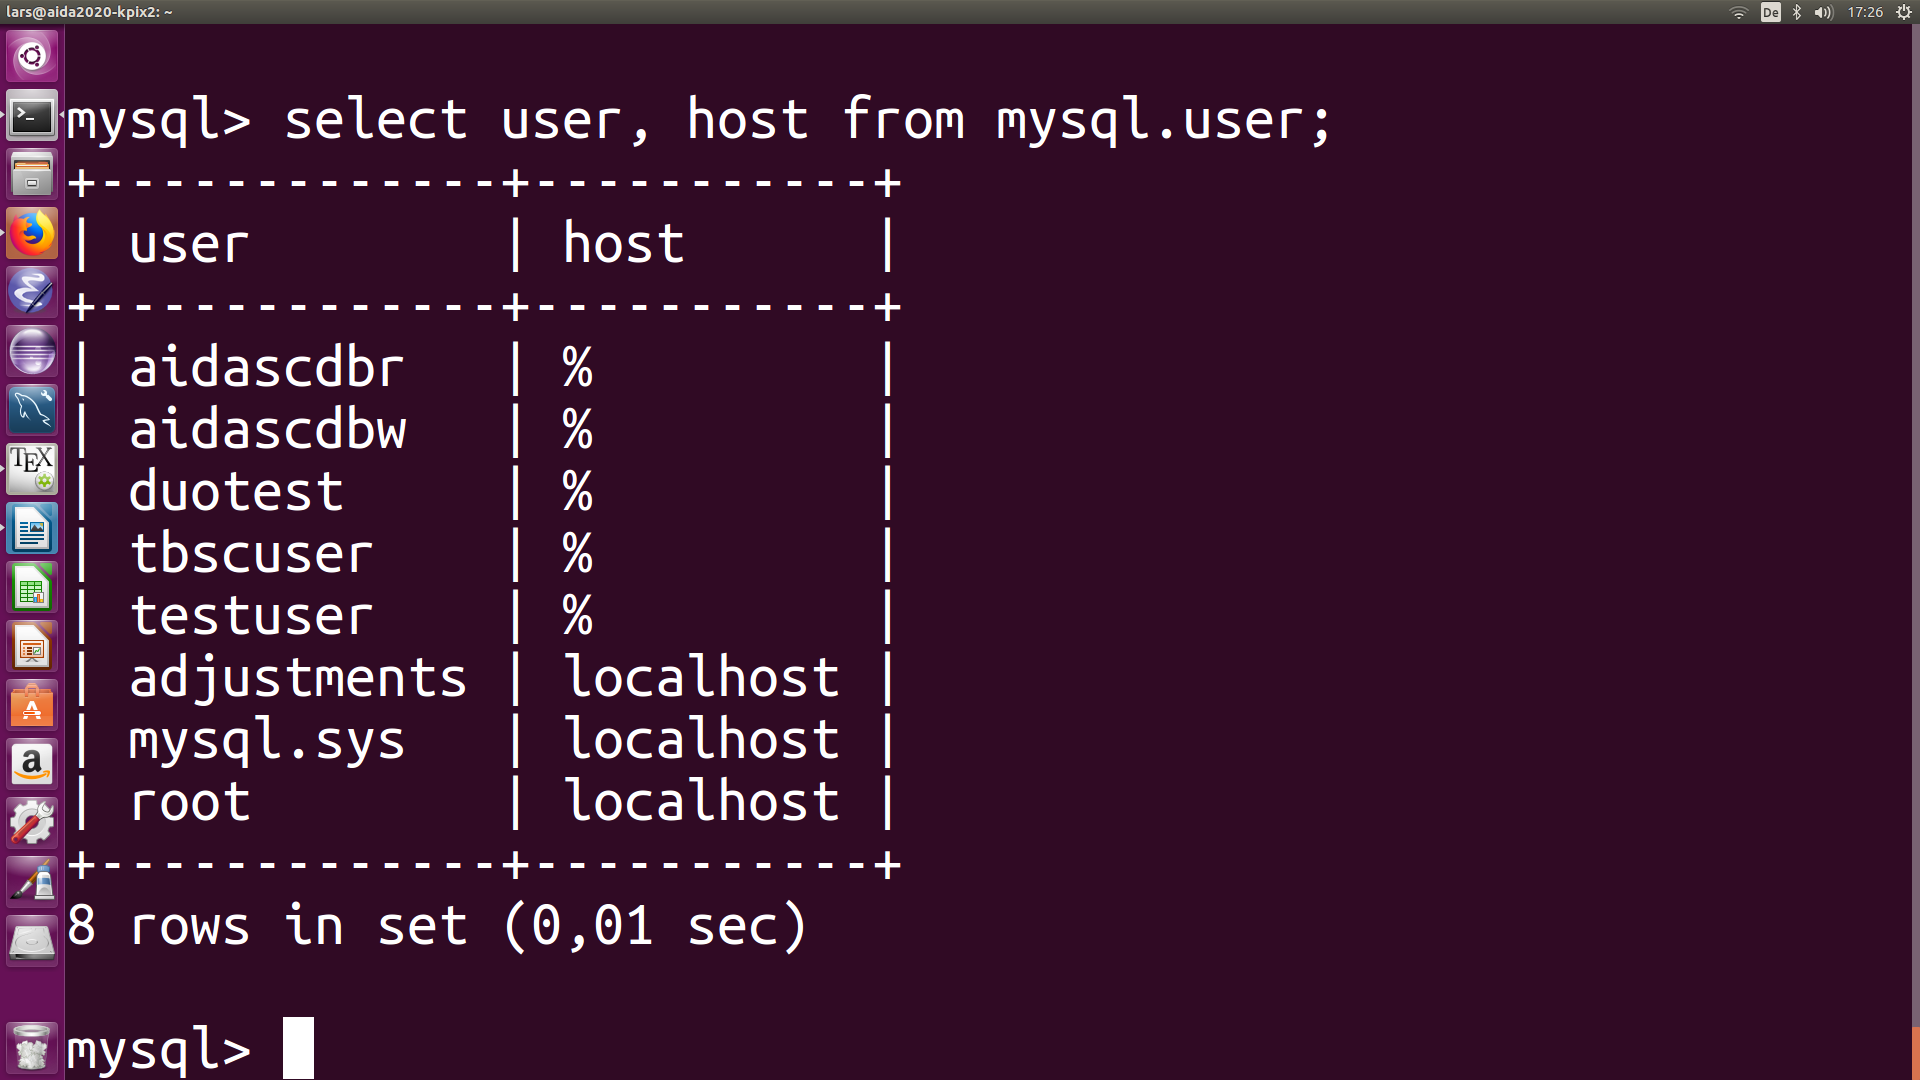
\includegraphics[trim={2cm 7cm 0cm 3cm},clip,width=0.65\textwidth]{mysqluser.png}
\caption{Check the access rights of which hosts to all the users in the MySQL, in this case, \texttt{aidascdbr} represents the read-only user prepared for EUDAQ2, while \texttt{aidascdbw} represents the write-only user prepared for AMR.}
\label{fig:mysql-user}
\end{figure}

%If there is no \% behind the username (Fig. 4) you are using, either use a different user with remote access or create a new user with this access: \\
\textbf{Notice}: \texttt{\%} is used as wild character, to allow the relevant useraccount to be accessed from multiple remove/local devices; for a certain user, it may have different privileges at different host, to check it, one can do (eg. aidascdbr):
\begin{lstlisting}[language=SQL]
mysql> SHOW GRANTS FOR 'aidascdbr'@'%';
\end{lstlisting}

To \texttt{GRANT} such \texttt{PRIVILEGES} to a certain user, you can use the following command:
%\colorbox{lightgray}{\texttt{mysql> GRANT ALL PRIVILEGES ON *.* TO 'USERNAME'@'\%' IDENTIFIED BY 'PASSWORD';}}\\
\begin{lstlisting}[language=SQL]
mysql> GRANT ALL PRIVILEGES ON *.* TO 'USERNAME'@'\%' IDENTIFIED BY 'PASSWORD';
\end{lstlisting}

Afterwards logged in as this user you can start to create your own database and tables: \\
\colorbox{lightgray}{\texttt{mysql> CREATE DATABASE \textit{Databasename};}}\\
Then you can choose to work with this database and create own tables and structure them: \\
\colorbox{lightgray}{\texttt{mysql> create table `tablename`(`counter` int unsigned zerofill auto\_increment,}}\\
\colorbox{lightgray}{\texttt{`timer` datetime NOT NULL, `value` double);}}\\



\subsection{ODBC}
The ODBC (Open DataBase Connectivity) is a general interface between different programms and databases. On the Windows PC has to be a ODBC/Connector for MySQL in a 32bit version [1] installed. \\
If this is installed a system DSN or user DSN can be created for a connection between the AMR software on the Windows PC and the MySQL database on the Linux PC. For creating a new DSN you have to open the ODBC data source administrator. \\ Click 'Add' under the register User or System DSN and continue with the configurations. \\
Name your new datasource and give the user with access rights to the MySQL database from multiple hosts. Choose the desired database for the transfared slow control data. For testing if your connection is working simply click on the 'Test' button.

\begin{figure} [H]
\centering
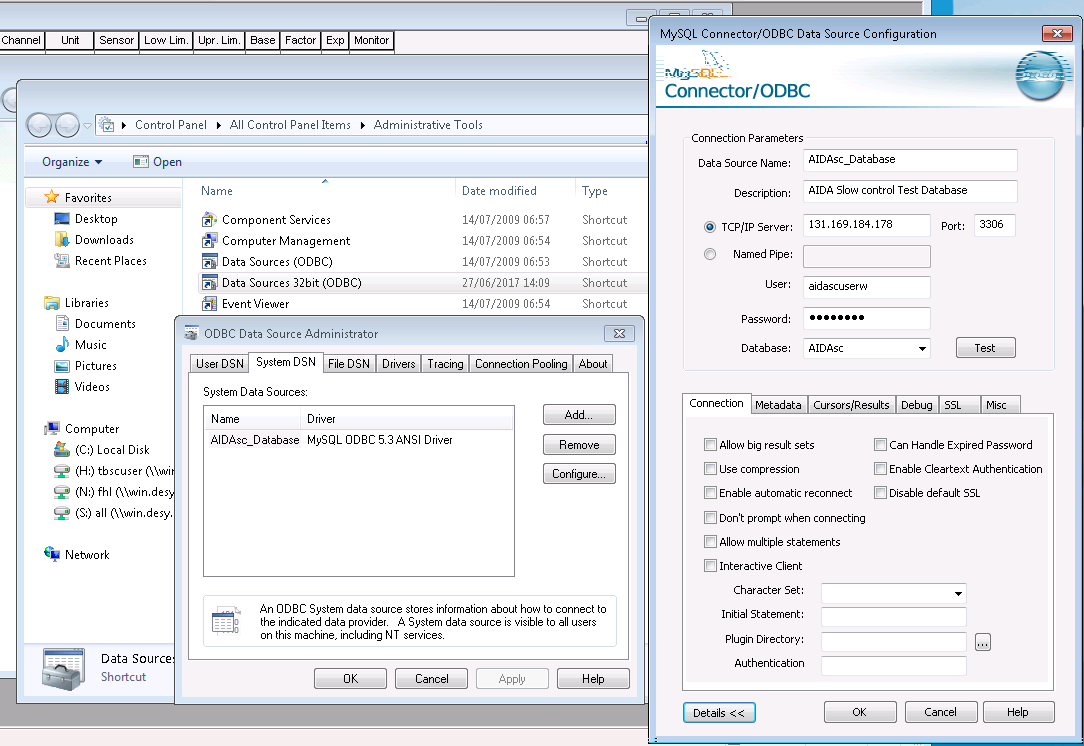
\includegraphics[width=\textwidth]{ODBC.png}
\caption{Adjust the properties of your ODBC DSN.}
\end{figure}

\subsection{unixODBC}
Thereby the EUDAQ framework can collect data from the MySQL database a unixDOBC has to be set up. It connects the different macros run by the EUDAQ RunControl with the MySQL database. There are two ways to create a new unixODBC connection. Before, please add this line to your shell setup (.bashrc): \\
\colorbox{lightgray}{\texttt{export ODBCSYSINI=/usr/local/etc}} \\ The first way is to change the odbcinst.ini file in the /etc directory of the Linux PC. A system DSN can just be added by the administrator or maintainer. \\
The second option to set up a unixODBC is to create a template file (Fig. 6) and add it to the DSNs of the PC. Specify the database, username and password, server and name the unixODBC in the squared brackets [2]. It is not of importance where the template file is stored. \\
To add the new unixODBC connection you only have to give the following command in the terminal [3]: \\
\colorbox{lightgray}{\texttt{odbcinst -i -s -f TemplateFileName}}\\
You can easy check if the ODBC has been added by showing all DSNs:\\
\colorbox{lightgray}{\texttt{odbcinst -q -s}}\\


\begin{figure} [H]
\centering
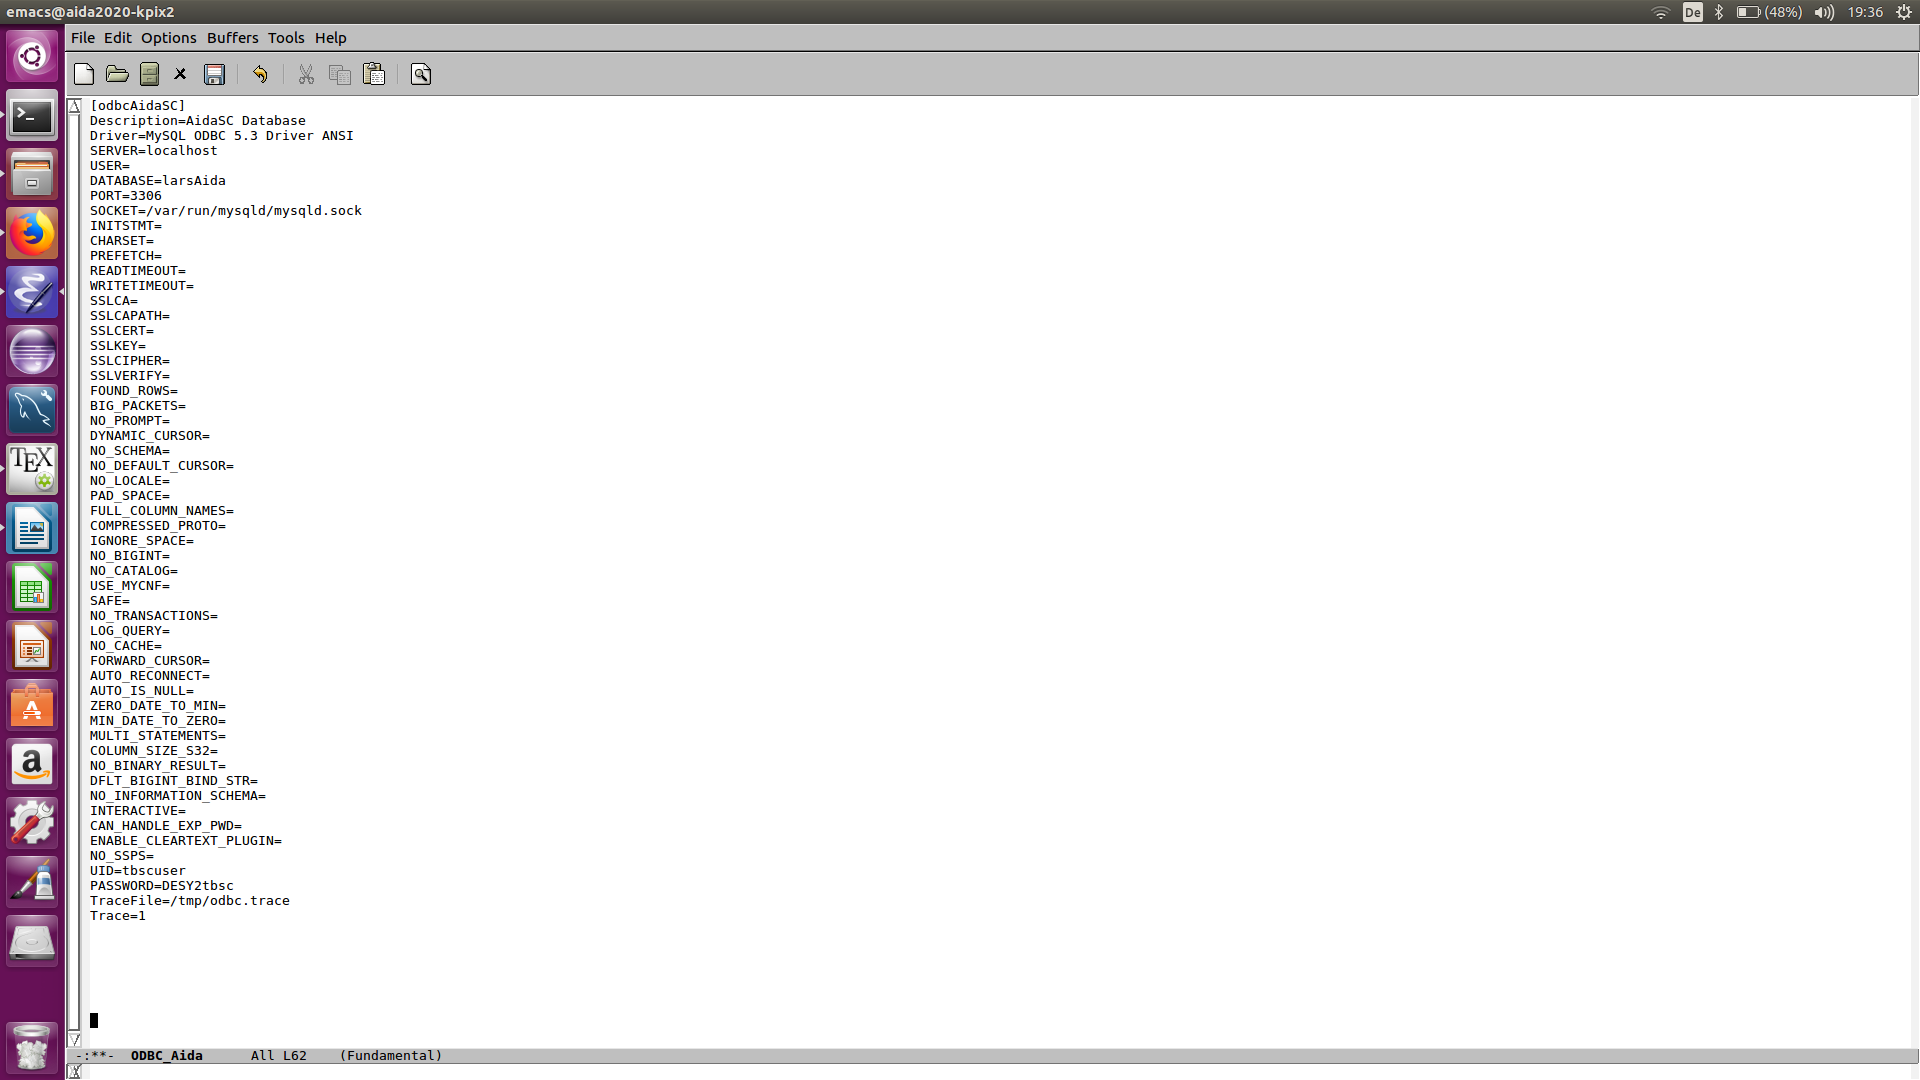
\includegraphics[trim={2.5cm 5cm 50cm 3.5cm},clip,width=7cm]{unixtemplate.png}
\caption{An example of a unixODBC template file.}
\end{figure}

\subsection{EUDAQ}
The EUDAQ framework was originally developed for the management of the Mimosa telescops (at DESY Duranta, Datura and Lycoris). The Slow Control System at DESY also uses the EUDAQ software to make it easyier to include to environmental parameters in other experimental datastreams. \\
The EUDAQ version used for the Slow Control System at DESY is stored and accessable in github [4]. To install this EUDAQ branch you follow the subsequent steps: \\
EUDAQ creates its own directory, you only have to run the command to install all files from the corresponding github repository: \\
\colorbox{lightgray}{\texttt{git clone https://github.com/MengqingWu/eudaq.git}} \\
After doing so you fetch the origin and check if the branch of your EUDAQ folder is mewu.master: \\
\colorbox{lightgray}{\texttt{git fetch origin}} \\
Check branch: \colorbox{lightgray}{\texttt{git branch}} \\
If the branch is not mewu.master, check into the right branch using: \\
\colorbox{lightgray}{\texttt{git checkout -b master orgin/mewu.master
}} \\
Befor continuing with the installtion make sure to have cmake or cmake-gui installed. You can do so by using:\\
\colorbox{lightgray}{\texttt{sudo apt-get install cmake}} or \colorbox{lightgray}{\texttt{sudo apt install cmake-qt-gui}}\\
Next of is the compilation with the makefiles. Create a /build directory under eudaq: \\
\colorbox{lightgray}{\texttt{mkdir build}} \\
And use the following command in this directory: \\
\colorbox{lightgray}{\texttt{cmake ..}} \\
Afterwards to finish the installation you use \\
\colorbox{lightgray}{\texttt{make install -j 4}}. \\

\section{Take Data}
When data taking there can occur multiple problems. The most common ones will be due to wrong connections in the conf file or because the AMR software is not polling. To illustrate the procedure of using the Slow Control System correctly there will be a short example:

\subsection{Operate the AMR software}
Open the AMR software in a remote Desktop via Ubuntu terminal(Fig. 7). \\
\colorbox{lightgray}{\texttt{xfreerdp /w:1600 /h:1000 /u:tbscuser /v:fhl-tb-sc01 /cert-ignore}} \\
make sure the ODBC connection is active, then click the red arrow in the top left corner. It should start blinking red and yellow when data is taken.

\begin{figure} [H]
\centering
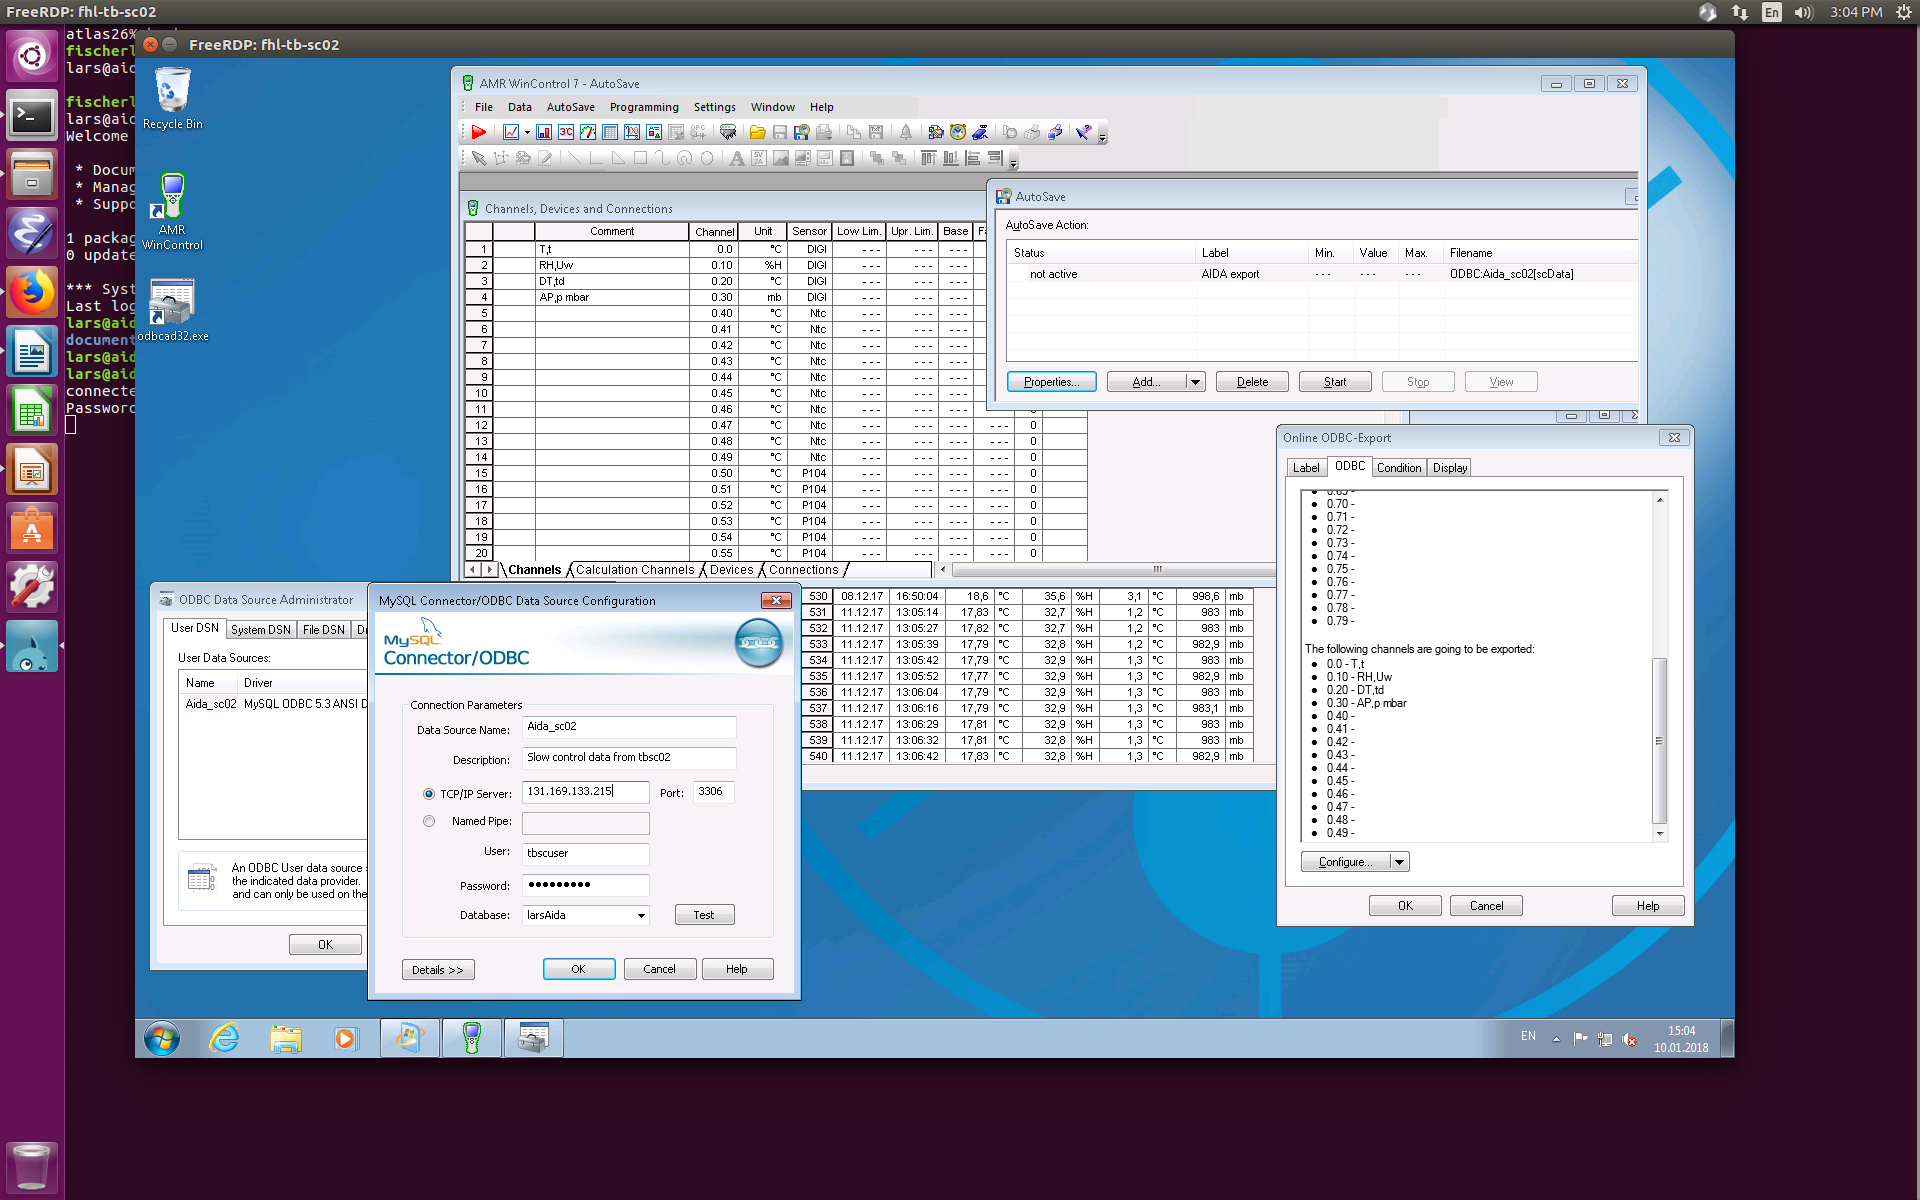
\includegraphics[trim={5cm 5cm 7cm 2cm},clip,width=\textwidth]{AMRSoftware.png}
\caption{AMR software (background) and ODBC connection (bottom left corner)}
\end{figure}

\subsection{Start EUDAQ}
To start EUDAQ go to the directory /bin and begin with running the GUI for the RunControl.\\
\colorbox{lightgray}{\texttt{./myeuRun}} \\
Use the Commands \\
\colorbox{lightgray}{\texttt{./euCliProducer -n tbscProducer -t tbsc}} \\
\colorbox{lightgray}{\texttt{./euCliCollector -n tbscDataCollector -t tbscDC}} \\
to start the Producer moduels and the DataCollector. All operations will be listed in the GUI of the RunControl.

\section{Integrate your own DataBase}
Section reserved to guide users to integrate their own DataBase to our slow control system.

\pagebreak
\section{References}
1: https://dev.mysql.com/downloads/connector/odbc/ \\
2: http://www.unixodbc.org/odbcinst.html \\
3: https://manpages.ubuntu.com/manpages/xenial/man1/odbcinst.1.html \\
4: https://github.com/MengqingWu/eudaq \\


\end{document}
